\subsubsection{Additions to webshop for assessment retake}
\begin{wrapfigure}[7]{l}{.4\textwidth}
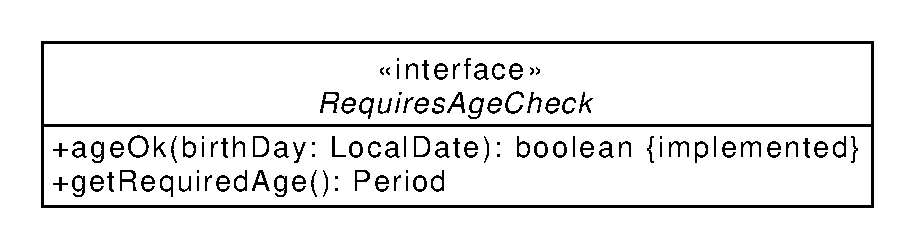
\includegraphics[width=.4\textwidth]{figures/booze.pdf}
\caption{\label{fig:booze}Product that requires age check.}
\end{wrapfigure}
The following additions have been made to the webshop in comparison to
the lab exercise:
\begin{description}
\item[Persist invoice] On sale, the Invoice information is persisted in the database or
  in the in-memory persistence  implementation. 
\item[Age check] Product has a sub class called \Code{Booze} which
  requires an age check on sale. From the class diagram in
  figure~\ref{fig:booze} you can see the relation of the product
  subcategory \Code{Booze}, the \Code{Product} class and the new
  interface \Code{RequiresAgeCheck}.
\end{description}
See the actual TODO list for the tasks these additions imply.


